\documentclass{beamer}




\mode<presentation>
{
  \usetheme{Warsaw}
  % or ...

  \setbeamercovered{transparent}
  % or whatever (possibly just delete it)
\useoutertheme{infolines}
}


\usepackage[english]{babel}
% or whatever

\usepackage[utf8]{inputenc}
% or whatever

\usepackage{times}
\usepackage[T1]{fontenc}
%\usepackage{listings}



\title[Diferencirana zasebnost] 
{Splošna definicija diferencirane zasebnosti}


\author[Metod Jazbec] 
{Metod Jazbec
\newline
\newline
Mentor: prof. dr. Aljoša Peperko}


\institute[FMF] 
{
  
  Fakulteta za matematiko in fiziko\\
  Univerza v Ljubljani
 }


\date[DS 2018] % (optional, should be abbreviation of conference name)
{Diplomski seminar, 2018}
% - Either use conference name or its abbreviation.
% - Not really informative to the audience, more for people (including
%   yourself) who are reading the slides online





% If you have a file called "university-logo-filename.xxx", where xxx
% is a graphic format that can be processed by latex or pdflatex,
% resp., then you can add a logo as follows:

% \pgfdeclareimage[height=0.5cm]{university-logo}{university-logo-filename}
% \logo{\pgfuseimage{university-logo}}



% Delete this, if you do not want the table of contents to pop up at
% the beginning of each subsection:
%\AtBeginSubsection[]
%{
%  \begin{frame}<beamer>{Kazalo vsebine}
%    \tableofcontents[currentsection,currentsubsection]
%  \end{frame}
%}


% If you wish to uncover everything in a step-wise fashion, uncomment
% the following command: 

%\beamerdefaultoverlayspecification{<+->}

\setbeamertemplate{caption}[numbered]
\begin{document}
%\lstset{language=Python}

\begin{frame}
  \titlepage
\end{frame}

\begin{frame}[allowframebreaks]{Kazalo vsebine}
  \tableofcontents
  % You might wish to add the option [pausesections]
\end{frame}


% Structuring a talk is a difficult task and the following structure
% may not be suitable. Here are some rules that apply for this
% solution: 

% - Exactly two or three sections (other than the summary).
% - At *most* three subsections per section.
% - Talk about 30s to 2min per frame. So there should be between about
%   15 and 30 frames, all told.

% - A conference audience is likely to know very little of what you
%   are going to talk about. So *simplify*!
% - In a 20min talk, getting the main ideas across is hard
%   enough. Leave out details, even if it means being less precise than
%   you think necessary.
% - If you omit details that are vital to the proof/implementation,
%   just say so once. Everybody will be happy with that.

\section{Uvod - opis teme}


\begin{frame}{Uvod}

  \begin{itemize}
  \item Diferencirana zasebnost - matematična definicija zasebnosti pri javni objavi ter rudarjenju podatkov.
 \end{itemize}
 \begin{columns}
 
\begin{column}{5.4cm}
\begin{figure}
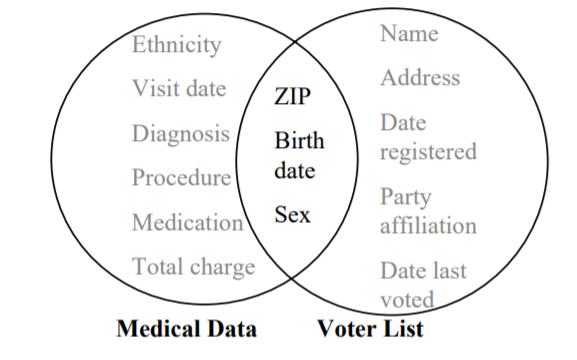
\includegraphics[width=5.4cm]{slika1} 
\caption{Metoda anonimizacije in napad s pomožno podatkovno bazo.}
\end{figure}
\end{column}

\begin{column}{5.4cm}
\begin{table}
\begin{center}
 \begin{tabular}{| c | c |} 
 \hline
 \textbf{Pacient} & \textbf{Diabetes}  \\ [0.5ex] 
 \hline
 Anja & 1  \\ 
 \hline
 Bojan & 1\\
 \hline
 Cene & 0 \\
 \hline
 Darja & 0  \\
 \hline
 Edi & 1  \\  
 \hline
\end{tabular}
\caption{Podatkovna baza z imeni pacientov in podatki o diabetesu.}
\end{center}
\end{table}
\end{column}

\end{columns}
\end{frame}


\section{Splošni podatkovni model}

\subsection{Podatkovna baza}
\begin{frame}{Podatkovna baza}
$(U, \rho)$ poljuben metrični prostor in $D \subseteq U$. Posamezni vnosi v opazovani podatkovni bazi so elementi množice $D$. Celotno bazo prikažemo z vektorjem \textbf{d} $= (d_{1}, ..., d_{n}) \in D^n$, kjer $d_{i} \in D$ predstavlja i-ti vnos oz. vrstico.
\newline
\newline
\begin{itemize}
\item Množico $U$ opremimo z Borelovo $\sigma$ -algebro, označimo jo z $\mathcal{A}_{U}$. 
\end{itemize}
\end{frame}

\begin{frame}{Sosednje podatkovne baze}
Pravimo da sta dve podatkovni bazi, \textbf{d}$= (a_{1},...,a_{n})$ in $\textbf{d'}= (b_{1},...,b_{n})$,  \textit{sosednji}, če se razlikujeta v natanko enem vnosu. Torej:
\begin{itemize}
\item obstaja $j\in\{1,...n\}$, da velja $a_{j} \neq b_{j}$,
\item za vsak $i\in\{1,...,n\} \setminus j$ velja $a_{i} = b_{i}$.
\end{itemize}
Sosednji bazi označimo z \textbf{d} $\sim$ \textbf{d\'}.
\end{frame}

\subsection{Poizvedba (query)}

\begin{frame}{Poizvedba}
\begin{itemize}
\item Poizvedba (query) je način pridobitve željenih informacij iz podatkovne baze (SQL ...).
\item Metrični prostor vseh možnih odgovor (angl. set of all possible responses) na posamezno poizvedbo  $(E_{Q}, \rho_{Q}, \mathcal{A}_{Q})$
\item  Poizvedba merljiva funkcija $Q: U^n \rightarrow E_{Q} $, torej $Q^{-1}(A) \in \mathcal{A}_{U^n}$ za vsako $A \in \mathcal{A}_Q$.
\end{itemize}
\end{frame}

\subsection{Odzivni mehanizem}

\begin{frame}{Odzivni mehanizem}
Naj bo $(\Omega , \mathcal{F}, \mathbb {P} )$ verjetnostni prostor. \textit{Odzivni mehanizem} (za izbran nabor poizvedb $\mathcal{Q}(n)$) je definiran kot družina slučajnih spremenljivk
\begin{equation}\label{odzivni}
 \{X_{Q,\textbf{d}} : \Omega \rightarrow  E_{Q} | Q \in  \mathcal{Q} (n), \textbf{d} \in D^n\} \tag{1}.
\end{equation} 
\begin{itemize}
\item Perturbacija podatkovne baze: 
\begin{equation}\label{odzivni2}
 X_{Q,\textbf{d}} = Q \circ Y_{\textbf{d}} \tag{2}
\end{equation} 
\item Perturbacija odgovorov na poizvedbo:
\begin{equation}\label{odzivni3}
X_{Q,\textbf{d}}=Z_{Q(\textbf{d})}\tag{3}
\end{equation} 
\end{itemize}
\end{frame}

\section{Definicija diferencirane zasebnosti}

\begin{frame}{Definicija diferencirane zasebnosti}
\begin{block}{Definicija (Diferencirana zasebnost za posamezno poizvedbo)}
Naj bo $\epsilon > 0$ in $0 \leq \delta \leq 1 $. Odzivni mehanizem je $(\epsilon, \delta)$-diferencirano zaseben za poizvedbo $Q$, če za vse $\textbf{d} \sim \textbf{d'} \in D^n$  in za vse $A\in\mathcal{A}_{Q}$ velja 
\begin{equation}\label{diferen}
\mathbb{P}(X_{Q,\textbf{d}} \in A) \leq e^\epsilon \mathbb{P}(X_{Q,\textbf{d'}} \in A) + \delta \tag{4}
\end{equation}
\end{block}
\begin{itemize}
\item Simetričnost definicije!
\end{itemize}
\end{frame}


\section{Omilitev zahtev definicije}

\subsection{Zadostne testne množice}
\begin{frame}{Zadostne testne množice}
\begin{block}{Izrek 1}
Naj bosta podana odzivni mehanizem \eqref{odzivni} in poizvedba $(E_Q, \mathcal{A}_Q, Q)$. Naj bo $S \subset \mathcal{A}_Q$ algebra in naj velja $\sigma(\mathcal{S}) = \mathcal{A}_Q$. Če \eqref{diferen} velja za vse $A \in \mathcal{S}$, potem velja za vse $A \in \mathcal{A}_Q$. 
\end{block}
\end{frame}

\subsection{Identična poizvedba}
\begin{frame}{Identična poizvedba}
\begin{itemize}
\item $I_n : D^n \rightarrow D^n$, $I_n$(\textbf{d})=\textbf{d} (javna objava celotne podatkovne baze).
\end{itemize}
\begin{block}{Izrek 2}
Naj bo odzivni mehanizem s perturbacijo podatkovne baze  $(\epsilon , \delta)$-diferencirano zaseben glede na identično poizvedbo $(U^n, \mathcal{A}_{U^n}, I_n)$. Potem sledi, da je tak mehanizem $(\epsilon , \delta)$-diferencirano zaseben glede na katerokoli poizvedbo $(E_Q, \mathcal{A}_Q, Q)$.
\end{block}
\begin{itemize}
\item  Posledica: mehanizmi oblike \eqref{odzivni2} so robustni na to, kolikokrat ponovimo določeno poizvedbo.
\end{itemize}
\end{frame}

\subsection{Poenostavitev na 1D baze}
\begin{frame}{Poenostavitev na 1D baze}
\begin{block}{Izrek 3}
Naj bo podana družina 1-dimenzionalnih diferencirano zasebnih mehanizmov $\{ Y_d: \Omega \rightarrow U | d \in D\}$. Velja torej
$$\mathbb{P}(Y_d \in A) \leq e^\epsilon \mathbb{P}(Y_d \in A) + \delta$$ 
za vse $d,d' \in D, A \in \mathcal{A}_D$. Če definiramo n-dimenzionalni odzivni mehanizem kot $Y_{\textbf{d}} (\omega) = (Y_{d_1} (\omega) , ... , Y_{d_n} (\omega))$, potem sledi, da je tudi ta diferencirano zaseben:
$$\mathbb{P}(Y_{\textbf{d}} \in A) \leq e^\epsilon \mathbb{P}(Y_{\textbf{d'}} \in A) + \delta$$
za vse $\textbf{d} \sim \textbf{d'} \in D^n, A \in \mathcal{A_{D^n}}$.
\end{block}
\begin{itemize}
\item Uporaba na diskretnem metričnem prostoru.
\end{itemize}
\end{frame}

\section{Primeri diferencirano zasebnih mehanizmov}
\begin{frame}{Laplaceov mehanizem na numerične podatke}
\begin{itemize}
\item  $D \subset \mathbb{R}$, kompakten. 
\item $L: \Omega \rightarrow \mathbb{R}$ Laplaceovo porazdeljena slučajna spremenljivka s parametroma $(0,b), b > 0$. 
Verjetnostna gostota ima potem obliko $f(x)=\frac{1}{2b}e^{-\frac{|x|}{b}}$.  
\item Za vsak $d \in D$ potem definirajmo 1-dimenzionalni mehanizem kot  $Y_{d}(\omega) = d + L(\omega)$. 
\item Parameter b izberimo tako da 
$$b\geq \frac{diam(D)}{\epsilon - \log(1-\delta)}.$$
Potem sledi, da je vsak n-dimenzionalen mehanizem oblike $Y_{\textbf{d}} (\omega) = (Y_{d_1} (\omega) , ... , Y_{d_n} (\omega))$ $(\epsilon, \delta)$ diferencirano zaseben za vsako poizvedbo $Q$. 
\end{itemize}
\end{frame}

\begin{frame}{Mehanizem na diskretne podatke}
\begin{itemize}
\item $D$ diskreten prostor, $|D| = m + 1$.
\item $Y_d$ mehanizem (slučajna spremenljivka): $\mathbb{P} (Y_d = d) = 1 - pm, \quad \mathbb{P}(Y_d = d') = p, \quad d, d' \in D$
\item $(\epsilon, \delta)-$diferencirana zasebnost bo dosežena natanko tedaj, ko $$p \geq \frac{1 - \delta}{m + e^{\epsilon}}$$
\end{itemize}
\end{frame}

\section{Natančnost odzivnih mehanizmov}
\begin{frame}{Natančnost odzivnih mehanizmov}
\begin{itemize}
\item $\gamma := max_{d\in D}\mathbb{E}[\rho(Y_d,d)].$ maksimalna pričakovana napaka danega mehanizma $Y_d$.
\end{itemize}
\begin{block}{Izrek 4}
Naj bo podana družina 1-dimenzionalnih diferencirano zasebnih mehanizmov $\{ Y_d: \Omega \rightarrow U | d \in D\}$. Potem velja $$\gamma  \geq (1-\delta)(\frac{diam(D)}{2(1+e^\epsilon)})$$
\end{block}
\begin{block}{Izrek 5}
Naj bo $D$ diskreten metrični prostor z $|D| = m + 1$ in $\kappa = \min_{d, d' \in D} \rho(d,d')$. Naj bo podana družina 1-dimenzionalnih diferencirano zasebnih mehanizmov $\{ Y_d: \Omega \rightarrow U | d \in D\}$. Potem velja $$\gamma  \geq (1-\delta)(\frac{\kappa m}{(m+e^\epsilon)}).$$
\end{block}
\end{frame}

\section{Dodatno o funkcijskih podatkih}

\begin{frame}{Dodatno o funkcijskih podatkih}
\begin{itemize}
\item $\textbf{d} = (d_1,...,d_n), \quad d_i \in \mathbb{R}^m$ ($d_i$ dobljeni iz porazdelitve z gostoto $f$)
\item Jedrna cenilka za gostoto:
$$
\hat{f}(x)=\frac{1}{n}\sum_{1}^{n}W\Big(\frac{||x-d_i||}{h}\Big), x \in \mathbb{R}^m
$$
($W$ jedrna funkcija, $h$ parameter dosega).
\item $D = \mathbb{R}^m, \quad E_Q \subseteq \mathbb{R}^D, \quad Q(\textbf{d}) = f_{\textbf{d}}, \quad X_{Q({\textbf{d}})} = \tilde{f}_{\textbf{d}}.$
\end{itemize}
\end{frame}

\begin{frame}{Hilbertovi prostori z reprodukcijskim jedrom}
\begin{block}{Definicija}
Naj bo $\mathcal{H}$ Hilbertov prostor, katerega elementi so funkcije oblike $f: X \rightarrow \mathbb{R}$ (pri tem je $X$ poljubna množica). Označimo z $L_x$ linearen funkcional, ki vsako funkcijo $f \in \mathcal{H}$ izvrednoti v $x$, torej $$L_x : f \rightarrow f(x).$$ Če je $L_x$ zvezen operator nad $\mathcal{H}$ za vsak $x \in X$, je $\mathcal{H}$ Hilbertov prostor z reprodukcijskim jedrom.
\end{block}
\begin{itemize}
\item $f(x) = L_x(f) = \langle f, K_x \rangle_{\mathcal{H}}, \quad \forall f \in \mathcal{H}$ (Riesz)
\item $K_x(y) = L_y(K_x) = \langle K_x, K_y \rangle_{\mathcal{H}}$
\item Reprodukcijsko jedro $K: X \times X \rightarrow \mathbb{R}, \quad K(x,y) := \langle K_x, K_y \rangle_{\mathcal{H}}$
\end{itemize}
\end{frame}

\begin{frame}{Gaussov proces}
\begin{block}{Definicija}
Gaussov proces, parametriziran z indeksno množico $T$, je slučajni proces $\{X_t : t \in T\}$, za katerega velja, da je za vsak končni nabor točk $t_1,...,t_n \in T$ slučajni vektor
$$
(X_{t_1},...,X_{t_n})
$$
porazdeljen večrazsežno normalno.
\end{block}

Gaussov proces je popolnoma določen s funkcijama povprečja  in kovariance: 
$$m(t) = \mathbb{E}X_t, \quad K(s,t) = Cov(X_s,X_t).$$
\end{frame}

\begin{frame}
\begin{block}{Izrek 6}
Naj bo $G$ trajektorija Gaussovega procesa s povprečjem 0 in kovariančno funkcijo $K$. Naj bodo $x_1,...,x_n \in D$. Naj bo matrika
$$
M(x_1,...,x_n) = 
 \begin{pmatrix}
  K(x_1,x_1) & \cdots & K(x_1,x_n) \\
  \vdots    & \ddots & \vdots  \\
  K(x_n,x_1) & \cdots & K(x_n,x_n) 
 \end{pmatrix}
$$
pozitivno definitna. Potem bo odzivni mehanizem 
$$
\widetilde{f}_{\textbf{d}} = f_{\textbf{d}} + \sqrt{2\log{\frac{2}{\delta}}} \frac{\Delta}{\epsilon}G
$$
$(\epsilon, \delta)$-diferencirano zaseben, ko bo veljalo
\begin{equation}\label{meja*}
\sup_{\textbf{d} \sim \textbf{d'}} \sup_{n < \infty} \sup_{(x_1,...,x_n) \in D^n} 
\bigg\|M^{-1/2}(x_1,...x_n)
\begin{pmatrix}
  f_{\textbf{d}}(x_1)-f_{\textbf{d'}}(x_1)  \\
  \vdots     \\
  f_{\textbf{d}}(x_n)-f_{\textbf{d'}}(x_n)
 \end{pmatrix}
\bigg\|_2 \leq \Delta. 
\end{equation}
\end{block}
\end{frame}

\begin{frame}
\begin{block}{Izrek 7}
Naj bo $f \in \mathcal{H}$, kjer je $\mathcal{H}$ Hilbertov prostor z reprodukcijskim jedrom $K$. Za vsako $x_1, ..., x_n$ končno zaporedje različnih točk v $\mathbb{R}^m$, za katero je matrika
$$
M(x_1,...,x_n) = 
 \begin{pmatrix}
  K(x_1,x_1) & \cdots & K(x_1,x_n) \\
  \vdots    & \ddots & \vdots  \\
  K(x_n,x_1) & \cdots & K(x_n,x_n) 
 \end{pmatrix}
$$
pozitivno definitna, velja
$$
\bigg\|M^{-1/2}(x_1,...x_n)
\begin{pmatrix}
  f(x_1)  \\
  \vdots     \\
  f(x_n)
 \end{pmatrix}
\bigg\|_2 \leq \|f\|_{\mathcal{H}}.
$$
\end{block}
\end{frame}

\begin{frame}
\begin{block}{Posledica}
Naj $E_Q$  podmnožica Hilbertovega prostora $\mathcal{H}$ z reprodukcijskim jedrom $K$, ki je enak kovariančni funkciji Gaussovega procesa (povprečje procesa naj bo enako 0). Če z $G$ označimo trajektorijo tega Gaussovega procesa, potem bo mehanizem 
$$
\widetilde{f}_{\textbf{d}} = f_{\textbf{d}} + \sqrt{2\log{\frac{2}{\delta}}} \frac{\Delta}{\epsilon}G
$$
$(\epsilon,\delta)-$diferencirano zaseben, ko bo veljajo 
$$
\sup_{\textbf{d} \sim \textbf{d'}} \| f_{\textbf{d}} -  f_{\textbf{d'}} \|_{\mathcal{H}} \leq \Delta.
$$
\end{block}
\end{frame}

\begin{frame}{Uporaba na primeru Gaussovega jedra}
\begin{itemize}
\item $\textbf{d} = (d_1,...,d_n), \quad d_i \in \mathbb{R}^m$ ($d_i$ dobljeni iz porazdelitve z gostoto $f$)
\item Cenilka za gostoto z Gaussovim jedrom: $f_{\textbf{d}}(x) = \frac{1}{n(2\pi h^2)^{d/2}} \sum_{i=1}^{n} exp\Big\{\frac{-\|x-d_i\|_{2}^{2}}{2h^2}\Big\},  \quad x \in \mathbb{R}^m$
\item $\textbf{d} \sim \textbf{d'}:$ $
(f_{\textbf{d}} - f_{\textbf{d'}})(x) = \frac{1}{n(2\pi h^2)^{d/2}} \Big(exp\Big\{\frac{-\|x-d_n\|_{2}^{2}}{2h^2}\Big\}-exp\Big\{\frac{-\|x-d_{n}^{\prime}\|_{2}^{2}}{2h^2}\Big\}\Big).
$
\item Za kovariančno funkcijo Gaussovega procesa $\{X_t : t \in T \}$ vzemimo Gaussovo jedro $K(x,y) = exp\{\frac{-\|x-y\|_{2}^{2}}{2h^2}\}$
\item $K(x,y) = K_x(y) = exp\{\frac{-\|x-y\|_{2}^{2}}{2h^2}\}, \quad f_{\textbf{d}} - f_{\textbf{d'}} = \frac{1}{n(2\pi h^2)^{d/2}} (K_{d_n}-K_{d_{n}^{\prime}})$
\item $\|f_{\textbf{d}} - f_{\textbf{d'}}\|_{\mathcal{H}}^{2} \leq  2 \Big(\frac{1}{n(2\pi h^2)^{d/2}}\Big)^2$
\end{itemize}
\end{frame}

\begin{frame}{Uporaba na primeru Gaussovega jedra}
\begin{figure}
\centering
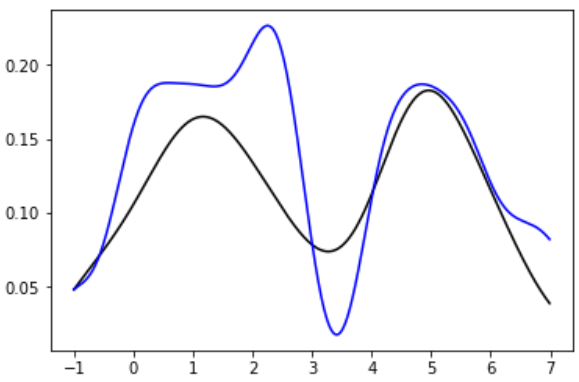
\includegraphics[width = 12cm, height = 6cm]{prva}
\caption{$\epsilon = 0.1, \delta = 0.1$}
\end{figure}

\end{frame}

\begin{frame}{Uporaba na primeru Gaussovega jedra}

\begin{figure}
\centering
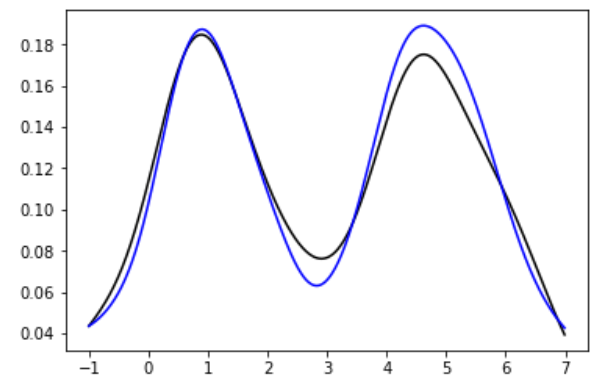
\includegraphics[width = 12cm, height = 6cm]{druga}
\caption{$\epsilon = 1, \delta = 0.1$}
\end{figure}
\end{frame}

\begin{frame}{Implementacija Laplaceovega mehanizma}
\begin{table}
\begin{center}
 \begin{tabular}{| c | c | c | c |} 
 \hline
 \textbf{$\epsilon$} & \textbf{$\delta$} & b   \\ [0.5ex] 
 \hline
 0.1 & 0.1 & 14589  \\ 
 \hline
 2 & 0.5 & 1112\\
 \hline
 11 & 0.7 & 245 \\
 \hline
\end{tabular}
\caption{b predstavlja parameter Laplaceove porazdelitve, povprečna razlika pa povprečje odstopanj diferencirano zasebnih podatkov od prvotnih. }
\end{center}
\end{table}
\begin{table}
\begin{center}
 \begin{tabular}{| c | c | c | c |} 
 \hline
 & povprečje & min & max  \\ [0.5ex] 
 \hline
 prvotni podatki & 2995 & 1504 & 4500  \\ 
 \hline
 (0.1 , 0.1) & 3402 & -111499 & 109729\\
 \hline
 (2, 0.5) & 2999 & -6110 & 11411 \\
 \hline
 (11, 0.7) & 2990 & 765 & 5360 \\
 \hline
\end{tabular}
\caption{Vrednosti nekaterih osnovnih poizvedb pri različnih vrednostih parametrov $(\epsilon, \delta)$. }
\end{center}
\end{table}
\end{frame}

\begin{frame}
\begin{table}[h]
\begin{center}
 \begin{tabular}{| c | c | c | c |} 
 \hline
($\epsilon, \delta$) & (0.1, 0.1) & (2, 0.5) & (11, 0.7)  \\ [0.5ex] 
 \hline
 spodnja meja za $\gamma$ & 640 & 89 & 0.0075  \\ 
 \hline
 dejanska največja napaka & 110600 & 7203 & 1803\\
 \hline
\end{tabular}
\caption{Spodnja meja največje napake $\gamma$ in dejansko opažena največja napaka pri različnih vrednostih parametrov $(\epsilon, \delta)$. }
\end{center}
\end{table}
\begin{itemize}
\item $\Delta Q = \max_{\textbf{d} \sim \textbf{d'}} \| Q(\textbf{d}) - Q(\textbf{d'}) \|_1$ (velika občutljivost identične poizvedbe).
\item Uber (sistem za SQL poizvedbe).
\item Skalirana metrika, problem?
\end{itemize}
\end{frame}
\begin{frame}{Implementacija mehanizma za diskretne podatke}
\begin{table}[!htb]
\begin{center}
 \begin{tabular}{| c | c | } 
 \hline
($\epsilon, \delta$) & verjetnost, s katero podamo pravi odgovor  \\ [0.5ex] 
 \hline
(0.1, 0.1) & 0.12  \\ 
 \hline
 (2, 0.5) & 0.57  \\ 
 \hline
 (7, 0.6) & 0.98  \\ 
 \hline
\end{tabular}
\caption{Rezultati mehanizma za diskretne podatke. }
\end{center}
\end{table}
\begin{table}[!htb]
\begin{center}
 \begin{tabular}{| c | c | c | c|} 
 \hline
($\epsilon, \delta$) & & &  \\ [0.5ex] 
 \hline
prvotni podatki & TX (114) & CA (102) & NY (63)  \\ 
 \hline
(0.1, 0.1) & TX (35) & OH (31) & CA (30)  \\ 
 \hline
(2, 0.5) & TX (68) & CA (62) & FL (45)  \\ 
 \hline
(7, 0.6) & TX (113) & CA (102) & NY (62)  \\ 
 \hline
\end{tabular}
\caption{Najpogostejše tri zvezne države v prvotnih podatkih in pri različnih vrednostih parametrov $(\epsilon, \delta)$. }
\end{center}
\end{table}
\end{frame}

\begin{frame}{Implementacija mehanizma za diskretne podatke}
\begin{table}[!htb]
\begin{center}
 \begin{tabular}{| c | c | c | c|} 
 \hline
($\epsilon, \delta$) & (0.1, 0.1) & (2, 0.5) & (7, 0.6)  \\ [0.5ex] 
 \hline
 spodnja meja za  $\gamma$ & 0.879 & 0.432 & 0.016  \\ 
 \hline
 dejanska največja napaka & 0.880 & 0.437 & 0.018\\
 \hline
\end{tabular}
\caption{Podatki o spodnjih mejah pri diskretnih podatkih. Dejanska največja napaka je tu izračunana kot razmerje med številom nepravilnih odgovorov ter številom posameznikov v bazi. }
\end{center}
\end{table}
\end{frame}




















% All of the following is optional and typically not needed. 
%\appendix
%\section<presentation>*{\appendixname}
%\subsection<presentation>*{For Further Reading}
%
%\begin{frame}[allowframebreaks]
%  \frametitle<presentation>{Viri in literatura}
%    
%  \begin{thebibliography}{10}
%    
%
%    
%  \beamertemplatearticlebibitems
%  % Followed by interesting articles. Keep the list short. 
%
%  \bibitem{Someone2000}
%    Naoise Holohan, Douglas J. Leith, Oliver Mason
%    \newblock Differential privacy in metric spaces: Numerical, categorical and functional data under the one roof
%    \newblock {\em Information Sciences, Volume 305}, 256-268, 2015.
%  \end{thebibliography}
%\end{frame}

\end{document}
